%%%%%%%%%%%%%%%%%%%%%%%%%%%%%%%%%%%%%%%%%%%%%%%%%%%%%%%%%%%%%%%%%%%%%%%%%%
%
% TRS - Physics -- LaTeX Source 
%
% $Id: trsPhysics.tex,v 1.1 1999/03/12 11:46:10 lasiuk Exp $
%
% Author: 1st version by brian
%
%%%%%%%%%%%%%%%%%%%%%%%%%%%%%%%%%%%%%%%%%%%%%%%%%%%%%%%%%%%%%%%%%%%%%%%%%%
%
% $Log: trsPhysics.tex,v $
% Revision 1.1  1999/03/12 11:46:10  lasiuk
% subsection of the reference manual
%
%%%%%%%%%%%%%%%%%%%%%%%%%%%%%%%%%%%%%%%%%%%%%%%%%%%%%%%%%%%%%%%%%%%%%%%%%%
\documentclass{article}
%
\usepackage{graphicx}
\usepackage{amsmath}
\usepackage{subfigure}
%\usepackage{../ucla/smallcap}  
%
\setlength{\textwidth}{5.5in}
%
\begin{document}

%%%%%%%%%%%%%%%%%%%%%%%%%%%%%%%%%%%%%%%%%%%%%%%%%%%%%%%%%%%%%%%%%%
\begin{center}
\thispagestyle{empty}
\flushbottom
\begin{flushright}  
  {\LARGE YRHI-99-29}
\end{flushright}

\vspace{2cm}

  {\LARGE \bf The Physics of the TPC Response Simulator}

  \vspace{1cm}

  {\large brian.lasiuk@yale.edu}

  \vspace{5cm}

  %Abstract
%  {\bf \underline{Abstract}}
\end{center}
  
  \vspace{1cm}

  \begin{flushleft}
    A brief summary of the physics that is simulated in the TPC
    Response Simulator (TRS).  This is taken from the TRS manual
    and user guide.  This is intended to be a STAR Note in the future.
  \end{flushleft}

  \newpage
\pagenumbering{arabic}


\section{Overview and Design} \index{overview} \index{design}
\label{sec:design}

The {\bf TRS} design document\footnote{http://www.rhic.bnl.gov/STAR/html/comp\_l/simu/TpcRespSim/src/ps/TrsDesign.ps} 
sets out the design, requirements and philosophy of {\bf TRS}, as well as
the first simple description of the algorithms proposed for use in
the various processes that are modeled.

The initial prototyping
phase led to the development of two types of classes
that make up the core of the physics and simulation components of
{\bf TRS}:
%%%%%%%%%%%%%%%%%%%%%%%%%%%%%%%%%%%%%%%%%%%%%%%%%%%%%%%%%%%%%%%%%%%%%%%
\begin{itemize}
   \item {\bf Processes} -- physical processes that model an aspect of 
     the physics occuring
     in the chamber such as charge transport, wire chamber operation
     and signal generation.  These are defined in detail in 
     section~\ref{sec:processes}.
   \item {\bf Containers} -- structures which contain the various types and
     forms of data required in the time evolution of the simulation.
\end{itemize}
%%%%%%%%%%%%%%%%%%%%%%%%%%%%%%%%%%%%%%%%%%%%%%%%%%%%%%%%%%%%%%%%%%%%%%%

In the class design of the package, each physical process, 
as described above, was mapped to a single class, as were the containers.
This provides a simple factorization 
between processes which allows them to function independently of
one another.  It also allows the isolation of single processes
for detailed study independent of the effect of other
processes.  As an example, previous attempts to simulate the
behavior of a wire chamber use a parameterization (f) of a 
pad response function from empirical relations such as:
%%%%%%%%%%%%%%%%%%%%%%%%%%%%%%%%%%%%%%%%%%%%%%%%%%%%%%%%%%%%%%%%%%%%%
\begin{equation}
f(x) \sim  e^{-(x-x_{o})^{2}/(2 \sigma^{2})}
\label{eq:alephPRF}
\end{equation}
%%%%%%%%%%%%%%%%%%%%%%%%%%%%%%%%%%%%%%%%%%%%%%%%%%%%%%%%%%%%%%%%%%%%%
where $\sigma$ incorporates terms which depend on the orientation of the
trajectory of a particle, the transport properties
of ionization through a gaseous medium, pad plane geometry, 
electronics properties, etc.  As such it is very difficult to isolate
the effects of a specific process, and parameters which affected
by many different processes result. This reduces the physical significance
of tunable parameters and while this may be fine for large scale production
of data, for understanding of the effects of physical processes, it is
not very useful.  This does not need to be the case since
the physics processes important in the operation of a TPC are
independent of not only the granularity of the simulation but also
the level of detail of the simulation.  As an example, one needs to
transport the ionization to the read-out plane independent of whether 
it is a single electron or segment of charge, however the detail of
whether one calculates the drift velocity at every point on a fine
mesh grid and propagate the charge across the grid, or do a simple
projection of the charge onto the pad plane.  As such, the above processes
can define an interface from which the {\em FAST}  parameterizations
and the {\em SLOW} microscopic simulation can utilize.  This allows
the use of the same code and interface with only a 
switch (or flag) which can be used to set the detail of
the simulation.  This allows the same infrastructure to handle
various levels of detail without resorting to separate packages for each.
Rather the same interface will mean the same function names
will be called, with only the implementations which vary.

As such, the {\bf processes} are the actual physical events that occur 
inside the chamber
and operate on data which are stored in {\bf containers}.  Thus a general
practice was followed that input data would be passed to a {\bf process} class
via a {\bf container} and the processor would either
mutate the data within the containers or produce data that would
be stored more naturally in a new or separate {\bf container} for the next
physics process.  As such, although the functions of these two types
of classes fulfill two different needs within the package, the relation
between them is very close.  These relations are explained in terms of
very physical means in the following two sections 
(sections~\ref{sec:processes} and \ref{sec:dataContainers}),

\subsection{Physical Processes}
\label{sec:processes}

There are four main types of {\bf processes} that were identified 
as being necessary to model in order to reproduce the operation of 
a TPC in {\bf TRS}.  When discussing the mode of operation of a TPC 
they become evident:
%%%%%%%%%%%%%%%%%%%%%%%%%%%%%%%%%%%%%%%%%%%%%%%%%%%%%%%%%%%%%%%%%%%%%%%%
\begin{itemize}
  \item {\em Ionization Transport} -- charge transport of the ionization.
    deposited in the active region to the readout chambers.
  \item {\em Charge Collection} -- electron/ionization collection on the
    sense wires of the multi-wire proportional chamber (MWPC).
  \item {\em Analog Signal Generation} -- charge induction on the pad plane and
    the generation of the time evolution of the analog signals on the pads.
  \item {\em Digital Signal Generation} -- Digital conversion of analog signals.
\end{itemize}
%%%%%%%%%%%%%%%%%%%%%%%%%%%%%%%%%%%%%%%%%%%%%%%%%%%%%%%%%%%%%%%%%%%%%%%%
A brief overview of the processes are given below, and more detailed
remarks are given in section~\ref{sec:simulationProcedure}.

\subsubsection{Ionization Decomposition and Transport}
\label{sec:ionizationTransport}

The ionization transport takes the charge deposited in an active volume
within a TPC detector and transports it through the field cage structure of
the TPC to the read-out plane.  The charge which is deposited can either
be generated externally, by GEANT \index{GEANT} or internally
given knowledge about parameters of the the fill gas in the chamber such
as the mean free path and ionization potential.

In the most common mode of operation, the ionization of the particle 
tracks will be described
by GEANT, which will provide the amount of energy deposited (dE) 
over a given path-length (ds), by a particle with a momentum $\vec{p}$.
Given the average ionization potential of the gas, the total number of 
electrons can be calculated such that the transport can be done at the
segment level (dE) or the single electron level.  This provides a mechanism 
which allows the possibility to distinguish between a detailed microscopic 
simulation and
a macroscopic parameterization; that is, the granularity of the simulation
can take on a range from the single electron level to a charge segment
containing many 10s of electrons.
By varying the length of the segment that is transported (and subsequently
processed), the granularity of the simulation can be varied.  The ionization
can then be distributed on the pad-plane according to the distributions
which characterize the effects of diffusion.  The role of the charge 
transporter is
to alter the x and y positions according to the transverse diffusions, the
z position to reflect the drift time, with the effects of longitudinal
diffusion folded in) and the amount of charge that actually reached the
read-out plane.

\subsubsection{Charge Collection and Amplification}
\label{sec:chargeCollection}

Once the electrons arrive at the read-out plane, they must be 
collected by the individual anode/sense wires of the multi-wire 
proportional chamber (MWPC).
This is where the avalanche process multiplies
the signal of several 10s of electrons to several 10$^{3}$-10$^{5}$, depending
on the potential on the wires.  This operation is somewhat of a hybrid as
it is really occurring within a container, however the processes
occur in the amplification
stage require the knowledge of the wire grid structure, and so the
processes are incorporated here for an efficient implementation.

\subsubsection{Analog Signal Generation}
\label{sec:analogSignalGeneration}

Once the charge is multiplied at the field wires of the MWPC, the
amount of charge induced on the pads produces an analog signal which
varies as a function of time.  These events can be modeled via two 
processes:
%%%%%%%%%%%%%%%%%%%%%%%%%%%%%%%%%%%%%%%%%%%%%%%%%%%%%%%%%%%%%%
\begin{itemize}
  \item charge induction on the pads.
  \item charge sampling by the electronics.
\end{itemize}
%%%%%%%%%%%%%%%%%%%%%%%%%%%%%%%%%%%%%%%%%%%%%%%%%%%%%%%%%%%%%%
Given
the amount of charge on the wires and the geometry of the pad plane,
the induced charge on any arbitrary pad can be calculated.  From this
quantity of charge, the signal at the output of the pre-amplifier/shaper
can be determined given the response (i.e.~transfer function) of the
analog electronics.  Although the
time evolution of the signal that is developed on the wires is nearly 
entirely due to the motion of the positive ions away from the wire, 
the number of electrons produced provides a measure of the total amount
of charge that is available to be induced on the pad plane.  The shaping
width of the electronics provide an estimate of the fraction of charge
that is really observed.  In reality only a fraction of the total charge 
is seen because of the
small mobility of the positive charged ions and it takes a long
time for the signal to finally decay (the famous 1/T tail).
As such the shaping 
properties of the analog electronics (i.e.~pre-amplifier and pulse shaping)
plays an important role in the amount of charge actually measured.
As such, given the total amount of charge induced on the pads, the
electronics will differentiate the signal, and be sensitive to a 
certain fraction of the total charge.  In the case of STAR, it is of
the order of 45\% of the charge.  This analog charge can then be distributed
into time bins modeling the behavior of the switch capacitor array (SCA)

\subsubsection{Digital Signal Generation}
\label{sec:digitalSignalGeneration}
\index{digital signal generator}

After the analog charge has been distributed into the time bins on
each pad, it can be digitized.  This is an important property which
is to be modeled because STAR uses a non-linear 8-bit ADC which
contains the information of a 10-bit linear scale.  Both the analog
and digital signal generation components operate on the signals
which are distributed in time bins, however there functions and operations
as well as the information contained differ enough to justify breaking 
the processes into two distinct types of processes.  The digital information
can be compressed much more and require a format that is accessible
via the {\em Data Decoder}.\footnote{see DAQ interface to Offline, M.~Shultz et al.}

\subsection{Data Containers}
\label{sec:dataContainers}
\index{containers}

The containers required for {\bf TRS} are essentially defined by 
the physics processes as described in section~\ref{sec:processes}.  Container
classes are used rather than simple data structures because it is
more simple to incorporate book-keeping and simple functions which
are closely matched to the structure of the container into a class.  
In essence the
containers establish a kind of {\em I/O} interface between the separate
processes and allow the same "physics framework" to exist, independent of
the granularity or detail of the simulation.  As a concrete example the
physics of the ionization transport of a charge segment through the
TPC field cage is independent of whether the segment in question is
a single electron or macroscopic charge cloud.  As such the containers
are designed in a very generic manner that would facilitate implementation
of the physics processes at various levels of detail and granularity.
The containers required for {\bf TRS} are:

\begin{itemize}
   \item {\em Charge Segment} -- the input to the program is an amount of
     energy (dE) deposited in a TPC volume with length (ds), by a
     particle of momentum $\vec{p}$.  In essence it is a object definition
     of a {\em g2t\_tpc\_hit}-like structure.
   \item {\em Charge Mini Segment} -- a fraction of a Charge Segment (above) 
     which can be, in the limit, the position of a single electron.
     This is transported to the read-out plane.
   \item {\em Wire Bin Entry} -- Position and charge of an ionization segment 
     (Charge Mini Segment)
     at the wire plane after the ionization transport.
   \item {\em Wire Histogram} -- all anode/sense wires which make
     up the MWPC which facilitates the charge collection.
   \item {\em Analog Signal} -- structure containing the time (centroid) and 
     amplitude of a signal on a pad.  This can function as storage 
     for both analog and digital signals
   \item {\em Analog Sector} -- contains analog signals on pads and is the
     main working structure for calculations involving the charge induced
     on the pads.
   \item {\em Digital Sector} -- contains digital signals on pads and contains the
     output data of the simulation.     
\end{itemize}

The containers and the processes are meant to be as independent
as possible and only overlap when concerns of efficiency over ride
the design guidelines.  The functions of the containers are described
in more detail below:

\subsubsection{Charge Segment}
\label{sec:chargeSegment}

The purpose of the slow simulator is to transform ionization
segments (usually produced by GEANT, or some type of external program)
to pixel, or Raw TPC Data.  As such the input will nominally
be a quantity of energy (dE) deposited by a track over a finite
path length (ds) at a coordinate ($\vec{x}$).  This information was
previously wrapped in two C/Fortran structures called {\em g2t\_tpc\_hit}
and {\em g2t\_tpc\_track}.  In the context of {\bf TRS} it is necessary, and
more convenient, to have this data wrapped in a class structure.  This
allows the same possibilities of data access as simple structures, however
the functionality goes beyond data encapsulation.  It also allows the
use of more flexible utilities such as the {\texttt StThreeVector} to
keep track of the position and momentum of track segment, as well as the
utilities these classes provide.  Furthermore operations that are
intrinsic to the segment itself such as rotation, fragmenting
(segment splitting) ({\em Note:} splitting requires knowledge
of the gas parameters as well), etc. can also be associated with
the object making
it more "complete".  These operations are necessary for rotating the
charge segment into the sector 12 reference frame of the TPC and
splitting the ionization into smaller segments to increase the granularity
of the simulation.

\subsubsection{Charge Mini Segment}
\label{sec:chargeMiniSegment}

The charge mini segment is a fragment of a charge segment (above) after it
has been split.  It can contain the complete charge segment or a 
fraction of it.  Each mini segment is distributed within the path length
of the charge segment (ds) onto a helical trajectory according to
the mean free path of the particle within the gas (medium).  
It is this mini segment on which
the charge transporter {\em process} will operate.  As such the relevant
data members are the position of the segment and the number of electrons.
Access and set functions are provided so that the transporter has read and
write access to these quantities.  

\subsubsection{Wire Bin Entry}
\label{sec:wireBin}

Once the charge reaches the anode wire grid it must be collected on
the sense/anode wires.  In order to distribute the ionization onto
the wires after diffusion effects are introduced 
(in the charge transporter), the ionization must be repackaged 
such that a specific quantity of
ionization can be assigned to a position on the anode wires.  Thus the
{\em wire bin entry} is made to collect an amount of charge, $q$ in the vicinity of
an anode wire at a position $\vec{x}$, which can be assigned to a wire.

\subsubsection{Wire Histogram}
\label{sec:wireHistogram}

The wire histogram is a class which models the charge collection on single
wires in a controlled manner; that is, charge is assigned through the
wire bin entry class.  The functionality of this class goes beyond
simply keeping track of the amount of ionization collected on a single
wire, but also possesses functions necessary to calculate gas gain
amplification of each cluster.  The reason this {\em ``process''} is associated
with a container is that the structure and layout of the wire grid,
which is necessary in the wire histogram is also necessary to be
able to do gas gain.  Thus instead of imposing overhead of redundant
class construction, it was incorporated here.  This is one of the advantages
of Object-Oriented design.  Each charge cloud can now be used to
induce a signal on the pad plane.

\subsubsection{Analog Signal}
\label{sec:analogSignal}

An electronic signal, regardless of it being analog or digital,
can be characterized by a pair of numbers which represents the
time (centroid) and total charge.  This class provides both access and
set functions to the data.  The storage of an
arbitrary signal is the purpose of this class.  In order for full
reconstruction of an analog form however, a functional form must also
be specified.  No matter, the final output of the {\bf TRS} package
is pixel data; that is a given amplitude at a given time which is
indexed by a pad-row and pad number.  Keeping the time allows the
flexibility of zero-suppressing any data with a negligible amplitude.
This structure is used to keep all the signals that are generated on the
pad plane, both analog and digital.  In this sense the term {\em analog}
is probably a misnomer, but it is foreseen in the future to introduce
another digital signal which does not require {\bf float} precision of
the stored values.  This should improve the storage requirements for
a single event.  

\subsubsection{Analog Sector}
\label{sec:sector}

The final output of the simulator is pixel data which is indexed
by pad-row, pad number, and perhaps time-bin.  The sector is
a container which can store an indeterminate number analog signals
indexed by these quantities.  As such after a specific charge is induced
onto the cathode pads, the analog sector keeps track of all intermediate
stages of calculation before digitization occurs.  
Please note that although both analog or
digital signals can be stored, only analog information is stored within
this structure.  The data is accessible either
by pad-row, or single pad indices.  Iterators are also provided within
the class to facilitate traversal of the structure.  

\subsubsection{Digital Sector}
\label{sec:digitalSector}

The final output of the simulator is pixel data which is indexed
by pad-row, pad number.  The digital sector is
a container which can store an indeterminate number of digital (8-bit) signals
indexed by these quantities.  The complete simulation of a complete
detector is 24 separate digital sectors.


\section{Mode of Simulation} \index{Simulation}
\label{sec:simulationProcedure}

This section describes in detail the processes that are
modeled, and the algorithms and methods that implement
the physics.
\subsection{Ionization Process}

The classes that deal with the raw ionization components within
the package is capable of manipulating ionization distributions
either generated from an external package 
(i.e.~GEANT), or given the momentum vector of a particle, generate 
the ionization in the active detector volume internally according 
to basic parameters of the fill gas in the chamber.

In normal operations, the ionization for each TPC sub-volume 
is taken according to the \texttt{g2t\_tpc\_hit} structures.  
This large segment is then broken up into pieces, according 
to an exponential distribution which has a mean value characterized
by the mean free path, between ionizing interactions, of a charged
particle within the gas.  This distribution, which specifies the
distance to the next interaction is given by:
%%%%%%%%%%%%%%%%%%%%%%%%%%%%%%%%%%%%%%%%%%%%%%%%%%%%%%%%%%%%%%%
\begin{equation}
        f(d) = K e^{-d/\bar{d}}
\label{eq:meanFreePath}
\end{equation}
%%%%%%%%%%%%%%%%%%%%%%%%%%%%%%%%%%%%%%%%%%%%%%%%%%%%%%%%%%%%%%%
where $\bar{d}$ is the mean free path.  It is derived from
the number of ionizing collisions which occur per unit
distance, $\bar{n}$.  The mean free path is then given by 1/$\bar{n}$.  
This gives rise to a distribution of ionizing interactions per
unit distance which is Poissonian in character.

At each interaction point a single ``primary'' electron is produced.  
These electrons will have an energy distribution given by 
the Rutherford scattering formula.  In the case of free $e^{-}e^{-}$ 
scattering (or at high momentum transfer where the binding energy
can be neglected), this implies an energy (E) distribution which
varies as E$^{-2}$.  Because the electrons are not, strictly speaking,
free  but rather bound to the atoms of the medium (in our case the TPC gas)
via a finite potential, there is a modification to this energy dependence
which is medium dependent.  This dependence has been measured experimentally
and can be quite accurately parameterized by a function of the
form E$^{-n}$.\footnote{see: H.~Fischle et al., NIM {\bf A301} (1991) 202;
  and B.~Lasiuk NIM {\bf A409} (1998) 402.}
For Ar, it is found experimentally that  
n=2 is a good approximation.  A similar behavior is expected for P10
which is 90\% Ar.  For lighter gases, n increases.  For
example, Ne requires n=2.2, and He, n=2.6.  This ``stiffening'' of the
primary electron energy spectrum is a consequence of the higher
binding energies of the lighter gases, however it has the desirable
effect of decreasing the width of the Landau distribution as
lower Z gases are used.  The reason is that although fewer secondary
electrons are produced, the spread in the energy distribution is smaller,
and this compensates for the degradation in statistics.
For this reason, resolution of dE/dx
measurements are nearly constant, independent of the gas
type used (to first order).
    
The energy dependence of the primary electrons is important because
it determines the amount of subsequent ionization that is generated.
For those primaries that have an energy above the ionization potential 
of the medium, which is typically the order of 10s of eV, subsequent 
electrons (secondaries) can be generated.  The number of secondaries 
N$_{sec}$ is then given by:
\begin{equation}
        N_{sec} = (E_{p} - I_{p})/W
\label{eq:secondary}
\end{equation}
where E$_{p}$ is the energy of the primary electron, I$_{p}$ is the 
ionization potential of the medium and W is the amount of energy necessary
to create an $e^{-}-ion$ pair. This is an ``effective'' quantity
which is very difficult to calculate from first principles and therefore
must be measured for each gas mixture individually.  It is found
that in most cases, except where the energy of the particle is very
small, the amount of energy required to produce an $e^{-}-ion$ pair
is independent of the energy of the incident particle.  This is seen
in figure~\ref{fig:W}.\footnote{From W.~Blum and L.~Rolandi
  {\em Particle Detection with Drift Chambers} Springer-Verlag 1994.}
%%%%%%%%%%%%%%%%%%%%%%%%%%%%%%%%%%%%%%%%%%%%%%%%%%%%%%%%%%%%%%%%%%%%%%
\begin{figure}[htb]
\begin{center}
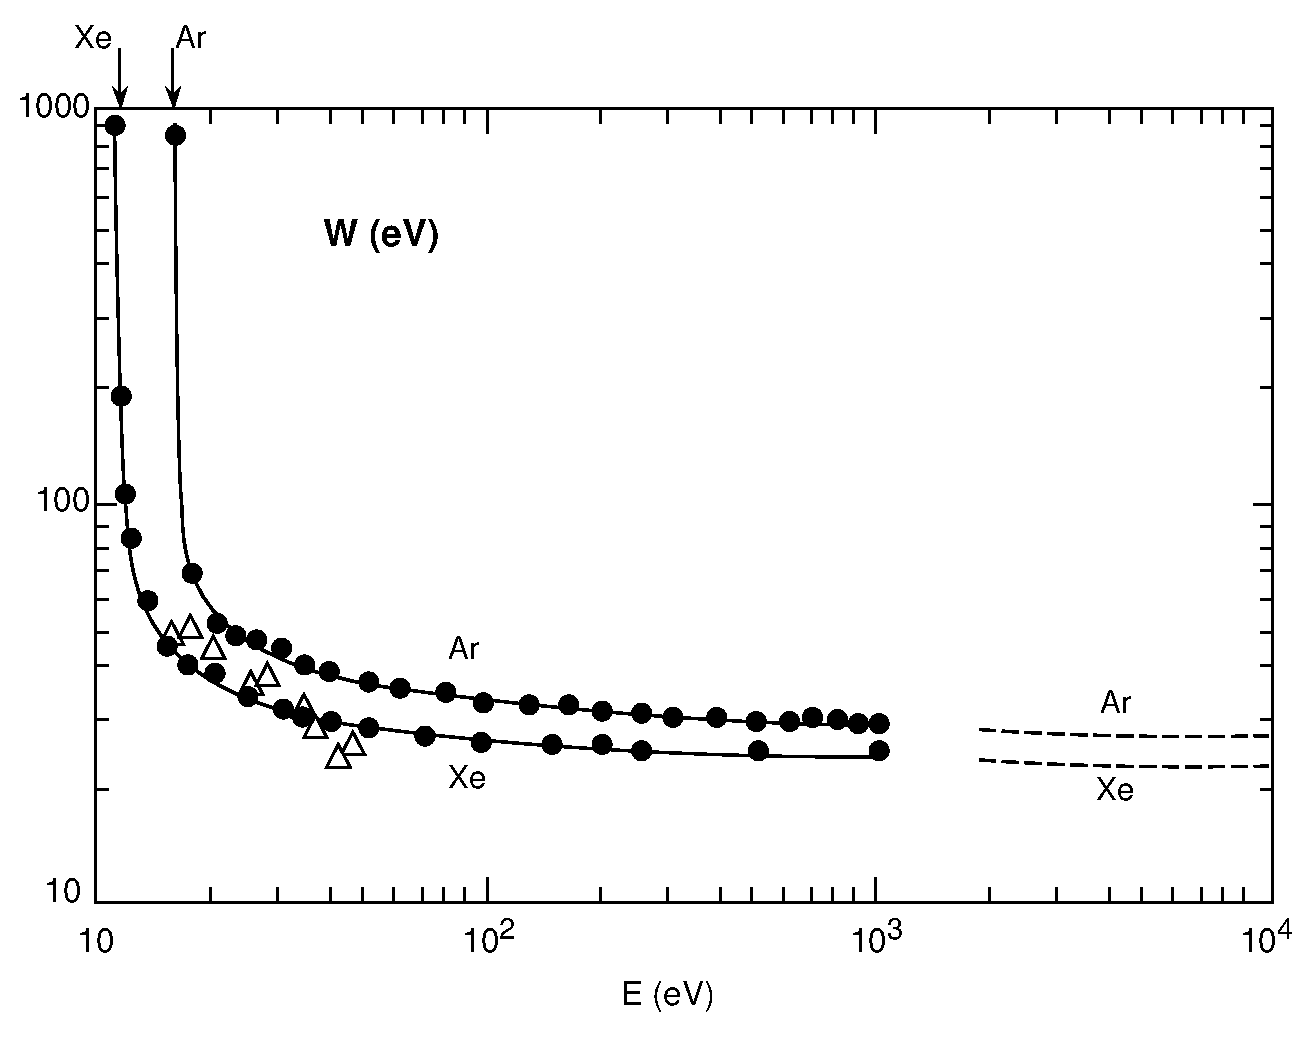
\includegraphics[width=.55\textwidth]{./pics/W.eps}
\caption{The average energy $W$ spent (in eV) for the creation
  of one electron-ion pair in Ar and Xe as a function of the incident
  energy of the ionizing particle (in this case, an electron).
  Dashed lines are extrapolations to higher energies.}
\label{fig:W}
\end{center}
\end{figure}
%%%%%%%%%%%%%%%%%%%%%%%%%%%%%%%%%%%%%%%%%%%%%%%%%%%%%%%%%%%%%%%%%%%%%%

The total number of electrons produced per interaction is
then given as the sum of the primaries and secondaries.
Thus calculating the number of electrons generated in a specific
length convolutes two distributions---a Poissonian which determines
the number of interactions, and an E$^{-n}$ which determines
the majority of the yield.  This procedure results in 
a Landau-like distribution---which is expected for the yield of 
ionization in a given path length.  Results for Ar and Ne are
shown in figure~\ref{fig:landauGases}.
%%%%%%%%%%%%%%%%%%%%%%%%%%%%%%%%%%%%%%%%%%%%%%%%%%%%%%%%%%%%%%%%%%%%%%
\begin{figure}[htb]
\begin{center}
\includegraphics[bbllx=33pt,bblly=150pt,bburx=569pt,bbury=698pt,width=.45\textwidth]{./pics/landauNe.ps}
\includegraphics[bbllx=33pt,bblly=150pt,bburx=569pt,bbury=698pt,width=.45\textwidth]{./pics/landauAr.ps}
\caption{Ionization statistics for primary, secondary, and total yield
  distributions for Ne (left panel) and Ar (right panel).  All yields
  are from a path length of 1.95~cm which is the pad length in the
  outer part of the TPC super-sector.}
\label{fig:landauGases}
\end{center}
\end{figure}
%%%%%%%%%%%%%%%%%%%%%%%%%%%%%%%%%%%%%%%%%%%%%%%%%%%%%%%%%%%%%%%%%%%%%%
Once the ionization is generated, or distributed into smaller
segments, it may then be transported to the multi-wire proportional
chamber (MWPC).

\subsection{Charge Transporter}

The charge, or ionization, in the segments that have been produced
must be transported to the sense (anode) wires of the MWPC for read-out.  
This transport is modeled in the {\bf Charge Transporter} component of 
{\bf TRS}, and three distinct processes are described:
\begin{itemize}
   \item E $\times$ B Effect.
   \item Transverse and Longitudinal Diffusion.
   \item Charge Loss {\em through}
   \begin{itemize}   
     \item Absorption through attachment (O$_{2}$).
     \item Gating Grid Transparency.
     \end{itemize}
\end{itemize}
and it is possible to control each process independently.
The charge transporter calculates the position of the charge
segment/electron at the z-plane of the anode/sense wire grid
and the amount of charge that arrives.  This charge must then
be collected and amplified on the anode wires.  In the
current implementation (i.e.~{\em FAST}) the charge is simply projected
in the z coordinate to the position of the anode/sense wire plane;
the underlying assumption that the ionization follows the $\vec{E}$
field lines and no distortions are visible.  This will be refined
in future versions.

\subsubsection{E $\times$ B Effect} {\em NOTE: not currently implemented!}
        
A misalignment between the electric and magnetic fields
or inhomogeneities in the magnetic field can
give rise to the ionization following trajectories which are not 
parallel to the $\vec{E}$ field lines.  This introduces distortions
into the trajectories of ionization left in the chamber.  These are
collectively known $\vec{E} \times \vec{B}$ distortions.
In the general case of a charged particle in the presence of an 
electric and magnetic field, it will not follow a trajectory
which is described by the Langevin equation:
%%%%%%%%%%%%%%%%%%%%%%%%%%%%%%%%%%%%%%%%%%%%%%%%%%%%%%%%%%%%%%%%%%%%
\begin{equation}
\frac{d{\bf v}}{dt} = \frac{q}{m}({\bf E} + {\bf v} \times {\bf B}) - \frac{1}{\tau} {\bf v}
\label{eq:lang}
\end{equation}
%%%%%%%%%%%%%%%%%%%%%%%%%%%%%%%%%%%%%%%%%%%%%%%%%%%%%%%%%%%%%%%%%%%%
where $q$ is the charge of the particle, $m$ is its mass, {\bf v} is 
its velocity, {\bf E} the electric (drift) field, {\bf B} the 
magnetic field, and $\tau$ is the average time between collisions 
with the molecules in the medium.  The last term is essentially 
a frictional force that limits the maximum average drift velocity.  
The steady state solution (i.e.~$\frac{d{\bf v}}{dt} = 0$) is given by:
%%%%%%%%%%%%%%%%%%%%%%%%%%%%%%%%%%%%%%%%%%%%%%%%%%%%%%%%%%%%%%%%%%%%
\begin{equation}
{\bf v} = \frac{\mu |{\bf E}| }{1 + \omega ^{2} \tau ^{2}} ( \hat{\bf E} + \omega  \tau   (\hat{\bf E} \times \hat{\bf B})  + \omega ^{2} \tau ^{2}(\hat{\bf E} \cdot \hat{\bf B} )\hat{\bf B})
\label{eq:exb}
\end{equation}
%%%%%%%%%%%%%%%%%%%%%%%%%%%%%%%%%%%%%%%%%%%%%%%%%%%%%%%%%%%%%%%%%%%%
where $\mu$ $($ $= \frac{e \tau}{m})$ is the electron mobility 
and $\omega$ $($ $= \frac{e B}{m})$ is the cyclotron frequency.  
Although in the ideal field cage structure of a TPC, the electric and
magnetic fields are parallel and the drift direction is defined
by the electric field vector.  Deviations from this idealization
introduces velocity components in the orthogonal directions.

Equation~\ref{eq:exb} allows the drift velocity to be calculated at any
arbitrary spatial point given knowledge regarding the electro-magnetic
field vectors and the mobility of electrons in the gas.
The distortions can then be modeled either by numerically
integrating the equation over the drift time of the ionization, or
parameterizing the displacement of the ionization in the plane
orthogonal to the $\vec{E}$ field.

\subsubsection{Diffusion}

The effects of diffusion are due to thermal motion of the molecules
in the gas and multiple scattering of
the ionization in the transport from the position of deposition
in the chamber to the read-out or sense wires on the pad plane.
While the mean position of a charge segment may be transported through
a volume with arbitrary electro-magnetic fields according to
equation~\ref{eq:exb}, its profile will broaden
in proportion to the drift length, or more appropriately,
the square root of its drift length.
It is possible to parameterize the evolution of the size of the
charge distribution (its width) in terms of a diffusion coefficient,
which is in principle,
different in the transverse ($\sigma_{T}$) and longitudinal ($\sigma_{L}$)
directions.  This distinction is important because the evolution
of the diffusion coefficient in the transverse direction also
depends on the presence of an magnetic field where it is
reduced according to:
%%%%%%%%%%%%%%%%%%%%%%%%%%%%%%%%%%%%%%%%%%%%%%%%%%%%%%%%%%%%%%%%%%%%
\begin{equation}
{\bf \sigma_{T}(B)} = \frac{\sigma_{T}}{1 + \omega ^{2} \tau ^{2}}
\label{eq:diffusion}
\end{equation}
%%%%%%%%%%%%%%%%%%%%%%%%%%%%%%%%%%%%%%%%%%%%%%%%%%%%%%%%%%%%%%%%%%%%
Once the charge segment/cloud is transported to the read-out plane,
each segment (or sub-component) can be distributed according to a
Gaussian (or any other) distribution characterized by a width derived
from the diffusion constants.  Increasing the granularity of the
charge distribution will better reproduce single electron statistical
fluctuations.

\subsubsection{Charge Absorption}
        
The absorption of charge is a complex process that
can be attributed to many different mechanisms.\footnote{Details
  contained in a soon to be added appendix.}
For our application we consider a simple parameterization of charge
attachment in a gas where trace amounts of oxygen are present.  The
probability (P) for attachment to occur in a specified drift time, t,
is given by:        
%%%%%%%%%%%%%%%%%%%%%%%%%%%%%%%%%%%%%%%%%%%%%%%%%%%%%%%%%%%%%%%%%%%%
\begin{equation}
             P(t) = 1 - e^{-At}
\label{eq:attach}
\end{equation}
%%%%%%%%%%%%%%%%%%%%%%%%%%%%%%%%%%%%%%%%%%%%%%%%%%%%%%%%%%%%%%%%%%%%
where A specifies an {\em attachment rate} given by:
%%%%%%%%%%%%%%%%%%%%%%%%%%%%%%%%%%%%%%%%%%%%%%%%%%%%%%%%%%%%%%%%%%%%
\begin{equation}
            A = P_{O_{2}} \cdot P_{M} \cdot C_{O_{2},M}
\label{eq:attachrate}
\end{equation}
%%%%%%%%%%%%%%%%%%%%%%%%%%%%%%%%%%%%%%%%%%%%%%%%%%%%%%%%%%%%%%%%%%%%
where P$_{O2}$ and P$_{M}$ are the partial
pressures of the oxygen and TPC gas respectively.
C$_{O2,M}$ specifies an {\em attachment coefficient} which
is a function of the gas in question and the reduced electric field (E/p).
For the case of STAR, a value of C = 10.2~$\mu$s$^{-1}$~bar$^{-2}$
has been deduced.\footnote{soon to be added appendix.}
To give an idea of the order of magnitude, for a concentration
of oxygen of 50~ppm and an ionization cloud drifting for
50~$\mu$s, the charge loss is expected to be approximately 2.5\%.
This charge loss can be applied at the single electron level or
an extended charge cloud where a fraction of the total is lost.

\subsubsection{Wire Grid Transparency}
        
As the charge enters the region of the wire grids in the
TPC, there is a non-zero probability that the charge may not
be transmitted due to the potential configuration on the wire
grids.  In the STAR TPC there are three wire grids:
%%%%%%%%%%%%%%%%%%%%%%%%%%%%%%%%%%%%%%%%%%%%%%%%%%%%%%%%%%%%%%%%%%%%
\begin{itemize}
   \item anode/sense---responsible for charge collection and
     amplification.
   \item zero/frisch---defines the boundary of the field cage and
     allows a sink for ion collection in the amplification process.
   \item gate---switch which controls passage of ionization from
     the active TPC volume to the sense/anode wire plane.
\end{itemize}
%%%%%%%%%%%%%%%%%%%%%%%%%%%%%%%%%%%%%%%%%%%%%%%%%%%%%%%%%%%%%%%%%%%%
The passage of ionization is controlled by the potential which
is applied to the gate wires.  Basically by setting the appropriate
potential on this grid, the drift $\vec{E}$ lines can be made to
terminate on the gating grid (zero transparency) or at the anode
wires (full transparency).  The transparency is the fraction of
lines that terminate on the anode wires compared to those that
terminate on the gating grid.

A general expression for the transparency of a mono-stable switched
gating grid was deduced such that
the full range from 0-100\% transmission can be
modeled.  It should be noted that the effects of a bi-polar switching
grid (which is the actual construction of the STAR-TPC) should not
influence the values at more than the $\sim$5\% level.
The expressions involved require only the geometry of the
wire grids and the voltages set on the gating grid
and high-voltage plane.  An example of the transmission curve
is shown in figure~\ref{fig:gridTransparency}.
%%%%%%%%%%%%%%%%%%%%%%%%%%%%%%%%%%%%%%%%%%%%%%%%%%%%%%%%%%%%%%%%%%%%
\begin{figure}[htb]
\begin{center}
\includegraphics[bbllx=14pt,bblly=137pt,bburx=569pt,bbury=701pt,width=.55\textwidth]{./pics/gridTransparency.ps}
\caption{Wire Grid Transparency Calculation for nominal wire potentials
  and STAR outer sector read-out chamber geometry.}
\label{fig:gridTransparency}
\end{center}
\end{figure}
%%%%%%%%%%%%%%%%%%%%%%%%%%%%%%%%%%%%%%%%%%%%%%%%%%%%%%%%%%%%%%%%%%%%%%

\subsection{Charge Collection}

According to the position of the charge segment/electron at the
anode wire plane, the ionization can be collected by the nearest wire.
The appropriate time delays for charge collection should a segment not
be projected directly on top of the wire position can be calculated.
Once the charge is assigned to a wire, the gas amplification can occur.

\subsubsection{Gas Gain Amplification at Sense Wires}

The process of gas amplification at the sense wires is modeled
by the Raether distribution,\footnote{see http://www.rhic.bnl.gov/STAR/html/comp\_l/simu/TpcRespSim/src/literature.html}
or, as it is denoted in Blum and Rolandi\footnote{W.~Blum and L.~Rolandi
  {\em Particle Detection with Drift Chambers} Springer-Verlag 1994.},
the Yule-Furry process which
describes the fluctuations in the amplification an amount of
charge q with an exponential distribution:
%%%%%%%%%%%%%%%%%%%%%%%%%%%%%%%%%%%%%%%%%%%%%%%%%%%%%%%%%%%%%%%%%%%%%%
\begin{equation}
          p(q) = \frac{1}{\bar{q}} e^{-q/\bar{q}}
\label{eq:raether}
\end{equation}
%%%%%%%%%%%%%%%%%%%%%%%%%%%%%%%%%%%%%%%%%%%%%%%%%%%%%%%%%%%%%%%%%%%%%%
Subsequent theoretical refinements to this simple expression which
were made in order to take into account effects like
the asymmetric growth of the avalanche profile as well as saturation
effects.  This resulted in several distribution, the Polya distribution
being the most popular.  It requires an additional parameter to supplement
the mean amplification ($\bar{q}$).  The effect of the additional parameter
is to suppress the small amplification factors.
As this parameter tends to zero, the Raether distribution is recovered.
Experimentally, perfectly exponential behavior is seen at
low to moderate gas gains (i.e.$<$10$^{4}$), in parallel plate geometry,
however at gas gains above 10$^{5}$, slight deformation from
exponential shape is observed.  This is probably
attributable to self-saturation effects which
become important because of space charge.  Since the TPC is generally
operated at low gas gains, the simple Raether distribution was
deemed acceptable, however the Polya function may be substituted
if there is need.

It should be noted that in TPC (or any drift chamber) operation,
the effect of the fluctuations in gas gain is to simply degrade the
attainable space-point resolution, and for this purpose the exact
functional form of the avalanche yields is not absolutely critical.
This degradation is the physics that the implementation of the gas-gain
fluctuations will attempt to address, and the Raether distribution should
be quite acceptable in this regard.

Once the charge has been amplified, the amount of charge induced on
the cathode pad plane can then be calculated.

\subsection{Analog Signal Generation}

The Analog Signal Generator has three main functions:
%%%%%%%%%%%%%%%%%%%%%%%%%%%%%%%%%%%%%%%%%%%%%%%%%%%%%%%%%%%%%%%%%%
\begin{itemize}
   \item Determine the charge induced on single pads from the charge
     ``collected'' on the anode wires.
   \item Sample the induced charge signals in time according to the
     electronics (i.e~pre-amplifier/shaper) response.
   \item Distribute the \underline{\bf analog} charge into time bins
     according to the parameters of the switched capacitor array (SCA).
   \end{itemize}
%%%%%%%%%%%%%%%%%%%%%%%%%%%%%%%%%%%%%%%%%%%%%%%%%%%%%%%%%%%%%%%%%%

\subsubsection{Charge Induction}

The charge induced on a grounded pad plane by a point charge $q$ located
a distance $d$ above the plane can be calculated by the method of
images.  The charge density ($\sigma$) on the plane is given by:
%%%%%%%%%%%%%%%%%%%%%%%%%%%%%%%%%%%%%%%%%%%%%%%%%%%%%%%%%%%%%%%%%%
\begin{equation}
  \sigma (x,y) = \frac{1}{2 \pi} \frac{q d}{((x-x_{o})^{2} + (y-y_{o})^{2} + d^{2})^{3/2}}
\label{eq:imageQ}
\end{equation}
%%%%%%%%%%%%%%%%%%%%%%%%%%%%%%%%%%%%%%%%%%%%%%%%%%%%%%%%%%%%%%%%%%
where the charge $q$ is located at a position (x$_{o}$,y$_{o}$).  However
this expression is not the solution for the charge induced on the pad
plane of a wire chamber.  In the case of a MWPC the charge, which
is at the position of the anode wire, is generally surrounded by {\em two}
cathode planes---one from
above and one from below.\footnote{Also the charge is in the form of
  a line charge associated with a linear charge density, not a
  discrete point charge.}
Thus in order to calculate the charge density induced on the pad
plane, all higher order multi-pole terms must be incorporated.
This results in the following expression:
%%%%%%%%%%%%%%%%%%%%%%%%%%%%%%%%%%%%%%%%%%%%%%%%%%%%%%%%%%%%%%%%%%
\begin{equation}
\sigma (x,y) = \frac{1}{2 \pi} \sum_{n}^{\infty} \frac{(2n+1) q d}{((x-x_{o})^{2} + (y-y_{o})^{2} + ((2n+1) d)^{2})^{3/2}}
\label{eq:imageQ2}
\end{equation}
%%%%%%%%%%%%%%%%%%%%%%%%%%%%%%%%%%%%%%%%%%%%%%%%%%%%%%%%%%%%%%%%%%
Doing the sum, (and integrating over all y) yields a function
which describes the charge distribution induced on the
pad plane at a distance $x$ from the wire where $x_{o}$ is
the position of the charge $q$:
%%%%%%%%%%%%%%%%%%%%%%%%%%%%%%%%%%%%%%%%%%%%%%%%%%%%%%%%%%%%%%%%%%
\begin{equation}
\sigma(x,y) = \frac{q}{4 d \cosh(\frac{\pi (x- x_{o})}{2 d})}
\label{eq:endo1}
\end{equation}
%%%%%%%%%%%%%%%%%%%%%%%%%%%%%%%%%%%%%%%%%%%%%%%%%%%%%%%%%%%%%%%%%%
This function, an inverse hyperbolic cosine as shown in
equation~\ref{eq:endo1} is called an {\em Endo function}.  Note that the
derivation put no limits on the extent of the pad in the y direction
(i.e.~$\frac{w}{l}=0$).
The effect of finite geometry of segmented cathodes can be accounted
for with the addition of another parameter.  The same function can
be written in a form more instructive for our purposes:
%%%%%%%%%%%%%%%%%%%%%%%%%%%%%%%%%%%%%%%%%%%%%%%%%%%%%%%%%%%%%%%%%%
\begin{equation}
\sigma(x) = K_{1} \frac{1 - \tanh^{2}(\frac{\pi (x-x_{o})}{4 d})}{1 + \tanh^{2}(\frac{\pi (x-x_{o})}{4 d})}
\label{eq:endo2}
\end{equation}
%%%%%%%%%%%%%%%%%%%%%%%%%%%%%%%%%%%%%%%%%%%%%%%%%%%%%%%%%%%%%%%%%%
where K$_{1}$ is a normalization constant.  Equation~\ref{eq:endo2}
can be used to generalize the Endo function in order to account for
finite geometry effects of the segmented cathode pads.  That is, each
pad has a finite width/length ratio.  This can be accounted for with
the addition of another constant K$_{2}$:
%%%%%%%%%%%%%%%%%%%%%%%%%%%%%%%%%%%%%%%%%%%%%%%%%%%%%%%%%%%%%%%%%%
\begin{equation}
  F(x) = K_{1} \frac{1 - \tanh^{2}(\frac{\pi (x-x_{o})}{4 d})}{1 + K_{2} \tanh^{2}(\frac{\pi (x-x_{o})}{4 d})}
\label{eq:gatti}
\end{equation}
%%%%%%%%%%%%%%%%%%%%%%%%%%%%%%%%%%%%%%%%%%%%%%%%%%%%%%%%%%%%%%%%%%
This is the generalized solution to the distribution of
charge induced on a grounded pad plane by a point/line charge,
and is usually dubbed, the Gatti function.  The Gatti function
is most prevalently used for pad chamber responses.  Although
more accurate, the price that is paid is the increase in time
required to integrate equation~\ref{eq:gatti} over the rather
simple expression which can be deduced from the integral of~\ref{eq:endo1}
A comparison of the Gatti and Endo functions to a Gaussian
(for reference) are given in figure~\ref{fig:gatti}
%%%%%%%%%%%%%%%%%%%%%%%%%%%%%%%%%%%%%%%%%%%%%%%%%%%%%%%%%%%%%%%%%%%%
\begin{figure}[htb]
\begin{center}
\includegraphics[bbllx=18pt,bblly=146pt,bburx=563pt,bbury=691pt,width=.55\textwidth]{./pics/prfShape.ps}
\caption{Comparison of Gaussian, Endo, and Gatti functions for profiles
  of the pad-response-function.}
\label{fig:gatti}
\end{center}
\end{figure}
%%%%%%%%%%%%%%%%%%%%%%%%%%%%%%%%%%%%%%%%%%%%%%%%%%%%%%%%%%%%%%%%%%%%%%

For the case of the TPC, the quantity of interest is the total
amount of charge ($Q$) induced per pad which means one must integrate
these functions, which specify the charge density, according to the
pad dimensions.  Thus for a point charge (equation~\ref{eq:imageQ}),
the integral is:
%%%%%%%%%%%%%%%%%%%%%%%%%%%%%%%%%%%%%%%%%%%%%%%%%%%%%%%%%%%%%%%%%%
\begin{equation}
  Q = \frac{1}{2 \pi} \int_{yl}^{yu} \int_{xl}^{xu} dx dy \frac{q d}{((x-x_{o})^{2} + (y-y_{o})^{2} + d^{2})^{3/2}}
  \label{eq:imageQint}
\end{equation}    
%%%%%%%%%%%%%%%%%%%%%%%%%%%%%%%%%%%%%%%%%%%%%%%%%%%%%%%%%%%%%%%%%%
where $xl$ and $xu$ denotes the lower and upper bounds of
the pad in the x direction respectively.  Similarly $yl$ and $yu$
denotes the same in the y
direction.  Similar integrals can be constructed given any
arbitrary charge density ($\sigma$).  The advantage of using such functions
is that they allow the production of longer tails which have
non-Gaussian characteristics.  The tails are an important characteristic
to understand as they determine the efficiency of the ionization
collection which is very important in the
study of ionization collection for $\frac{dE}{dx}$ resolution.
Furthermore these integrals are well defined
given the the position of the charge and the coordinates
of the pads.  Thus charge induced on adjacent pads as well as rows
can be also be calculated quite simply in this formalism.
Illustrations of some of these
function are shown in figures~\ref{fig:gatti}.\footnote{For more
  details see: http://www.rhic.bnl.gov/STAR/html/comp\_l/simu/TpcRespSim/src/literature.html} 

%%%%%%%%%%%%%%%%%%%%%%%%%%%%%%%%%%%%%%%%%%%%%%%%%%%%%%%%%%%%%%%%%%%%
%\begin{figure}[htb]
%\begin{center}
%\includegraphics[bbllx=14pt,bblly=137pt,bburx=569pt,bbury=701pt,width=.55\textwidth]{}
%\caption{Comparison of Gaussian, Endo, and Gatti functions for PRF.}
%\label{fig:xxx}
%\end{center}
%\end{figure}
%%%%%%%%%%%%%%%%%%%%%%%%%%%%%%%%%%%%%%%%%%%%%%%%%%%%%%%%%%%%%%%%%%%%%%
Please keep in mind that the fact that the signal on the wire is
due almost exclusively to the motion of the charged ions {\bf away} from
the wire.  In order to calculate the total amount of charge induced
on the pad however, it is possible to use the number of electrons
as a quantity, even though they are not the physical reason for
the charge induction.  This point will be reiterated in the electronics
response of this description.

\subsubsection{Sample the Signal in Time}

Once the amount and centroid of the charge distribution
on each pad is determined, this charge can be sampled in
time corresponding to the analog electronics response.
The signals are generated by super-imposing each analog signal
from each avalanche which induces a signal on the pad plane.
This allows the shaping
time of the electronics can be varied independently of
the width of the pad response function which is the strength
of this simulation methodology.  Currently four types of
sampling are possible:
%%%%%%%%%%%%%%%%%%%%%%%%%%%%%%%%%%%%%%%%%%%%%%%%%%%%%%%%%%%%%%%%%%
\begin{itemize}
  \item delta function.
  \item Symmetric Gaussian.
  \item Asymmetric Gaussian.
  \item Parameterized STAR response.
\end{itemize}
%%%%%%%%%%%%%%%%%%%%%%%%%%%%%%%%%%%%%%%%%%%%%%%%%%%%%%%%%%%%%%%%%%
A function also exists where a fractional scale of the total charge integral
can be added as an Undershoot/Unrestored baseline component in the
signal which has the effect of convoluting effects from the long 1/T tail.
This is an important point and one that actually blurs the line of
physics and simulation.  In reality the
time evolution of the signal that is developed on the wires is nearly 
entirely due to the {\bf motion of the positive ions} away from the wire.
This produces a signal with a long 1/T tail.  For the STAR geometry
the signal is $\sim$62~$\mu$s.  In order to make a detector faster,
the signal is differentiated after a characteristic time---the
shaping time of the pre-amplifier.  Although the detector response
becomes faster, the trade-off is that only a fraction of the total
charge is seen by the downstream electronics (i.e.~the ADC).  This
fraction $F$, is given by:
%%%%%%%%%%%%%%%%%%%%%%%%%%%%%%%%%%%%%%%%%%%%%%%%%%%%%%%%%%%%%%%%%%
\begin{equation}
  F = \frac{ln(1+\frac{t_{m}}{t_{o}})}{ln(1+\frac{t_{s}}{t_{o}})}
  \label{eq:fraction}
\end{equation}    
%%%%%%%%%%%%%%%%%%%%%%%%%%%%%%%%%%%%%%%%%%%%%%%%%%%%%%%%%%%%%%%%%%
where t$_{m}$ is the length of time the undifferentiated signal would
persist (i.e.~$\sim$62~$\mu$s), t$_{o}$ is the characteristic time
of the signal development (i.e.~$\sim$1~ns), and t$_{s}$ is the shaping
time of the pre-amplifier (i.e.~$\sim$180~ns).  For STAR this implies
the order of 45\% of the charge is distributed into time bins by the
SCA.  More importantly is that the signal shape is dominated very strongly
by the shaping properties of the electronics.  Thus the
long time response of the chamber is parameterized in the electronics
processing component of the simulator, rather than modeling the
motion of the positive ions.

The symmetric Gaussian response, with the effect of an unrestored baseline
due to under/over shoot is illustrated in figure~\ref{fig:baseline}
%%%%%%%%%%%%%%%%%%%%%%%%%%%%%%%%%%%%%%%%%%%%%%%%%%%%%%%%%%%%%%%%%%%%
\begin{figure}[htb]
\begin{center}
\includegraphics[bbllx=14pt,bblly=137pt,bburx=569pt,bbury=701pt,width=.55\textwidth]{./pics/baseline.ps}
\caption{Asymmetric Gaussian Electronics Response with pedestal suppressed
  showing both undershoot (top panel) and an under damped
  baseline restoration (bottom panel).}
\label{fig:baseline}
\end{center}
\end{figure}
%%%%%%%%%%%%%%%%%%%%%%%%%%%%%%%%%%%%%%%%%%%%%%%%%%%%%%%%%%%%%%%%%%%%%%
where the time evolution of a series of 20 signals, of identical
amplitude, are induced on a single pad.\footnote{More examples can
  be seen at: http://www.rhic.bnl.gov/STAR/html/comp\_l/simu/TpcRespSim/src/literature.html} 
The pulses are simply added using the principle of super-position.
The modeling of an unrestored baseline is very
important since the pulse height (actually the integral) of the
signal is used as a measure of the velocity of the particle
(via $\frac{dE}{dx}$ information).
An unrestored baseline due to undershoot can result in
an effective loss of charge in a high-multiplicity environment.  Conversely
an unrestored baseline due to under-damping will result in too much
charge being observed at large drift distances.  Both effects
will reduce the attainable resolution if not taken into account.  

Once the complete functional form of the signals induced on a pad
over the read-out period of the TPC electronics, the analog charge
can be distributed into discrete time bins. This sampling simulates
the behavior of the switched capacitor array (SCA) in the front-end
electronics.  This is done by integrating the amount of charge in
a time interval $\Delta$t, which is determined from the SCA sampling
frequency.  Chamber noise as well as electronic noise
can be added at this point.

\subsection{Digital Signal Generation}

Once the analog charge is distributed into time bins on the pads,
the digitization can occur.  This is currently a simple
conversion from voltage to ADC counts.  Other features
such as the addition of a pedestal
and non-linearities in the ADC can also be added.
In fact, any characteristic of the
digital electronics can be added and will be independent
of the analog signal sampling.  This is very close to
the way the front-end electronics are designed where the
digital and analog electronic components are separated.

\section{Physics Limitations}

There are still some components either not implemented,
or completely missing from TRS in its current form.  It
is hoped that these will be incorporated as the understanding
of TRS evolves.  Most critically is the noise.  Although some
preliminary work exists for this modeling, it has currently not
reached a mature enough state where it can be added.  Some obvious
short-comings are listed below.
%%%%%%%%%%%%%%%%%%%%%%%%%%%%%%%%%%%%%%%%%%%%%%%%%%%%%%%%%%%%%%%%%%%%
\begin{itemize}
  \item $\vec{E} \times \vec{B}$ in not tested although code exists
    and can be "plugged" in.
  \item Noise at the chamber and electronics level does not yet exist.
  \item A function (or look-up table) is needed for the non-linear ADC
    response.
  \item The pad geometry is not incorporating the fractional pads at the
    border of the sectors.
  \item The gas gain is currently independent of the wire and the
    position of the avalanche on the wire.
  \item Effects of space charge in the charge transport stage of the
    simulation.
  \item No positional dependence in the transparency of the gating grid
    exists.  Currently a constant transparency, independent of position
    is calculated.
\end{itemize}
%%%%%%%%%%%%%%%%%%%%%%%%%%%%%%%%%%%%%%%%%%%%%%%%%%%%%%%%%%%%%%%%%%%%

It is almost certain that as
experience is gained with the package, this list will be further
expanded, however the code is written in a flexible manner such that
these type of additions should be relatively straight forward.
\end{document}
